\documentclass[11pt,a4paper]{article}

\usepackage[utf8]{inputenc}
\usepackage[T1]{fontenc}
\usepackage{geometry}
\geometry{a4paper, margin=1in}
\usepackage{graphicx}
\usepackage{booktabs}
\usepackage{amsmath}
\usepackage{hyperref}
\usepackage{listings}
\usepackage{xcolor}

\definecolor{codegray}{rgb}{0.5,0.5,0.5}
\definecolor{codegreen}{rgb}{0,0.6,0}
\definecolor{codeblue}{rgb}{0,0,0.8}
\definecolor{backcolour}{rgb}{0.95,0.95,0.92}
\definecolor{tamugray}{HTML}{3C3C3C}

\lstdefinestyle{mystyle}{
    backgroundcolor=\color{backcolour},   
    commentstyle=\color{codegreen},
    keywordstyle=\color{magenta},
    numberstyle=\tiny\color{codegray},
    stringstyle=\color{codeblue},
    basicstyle=\ttfamily\scriptsize,
    breakatwhitespace=false,         
    breaklines=true,                 
    breakindent=0pt,
    captionpos=b,                    
    columns=fullflexible,
    frame=single,
    framesep=3pt,
    keepspaces=true,                 
    numbers=left,                    
    numbersep=6pt,                  
    postbreak=\mbox{\textcolor{codegray}{$\hookrightarrow$}\space},
    showspaces=false,                
    showstringspaces=false,
    showtabs=false,                  
    tabsize=2,
    xleftmargin=1.5em,
    framexleftmargin=1em
}
\lstset{style=mystyle}

\hypersetup{
    colorlinks=true,
    linkcolor=tamugray,
    filecolor=magenta,      
    urlcolor=blue,
    pdftitle={VisionOps Crew: A Multi-Agent Architecture for Computer Vision Operations},
    pdfpagemode=FullScreen,
}

\title{\textbf{VisionOps Crew: A Multi-Agent Architecture for Computer Vision Operations}\\[0.75em]
\large Coordinating Model Research, Dataset Curation, Runtime Inspection, Notebook Prototyping, and Artifact Generation}
\author{\textbf{Henry Ruiz, PhD} \\ Texas A\&M University \\ \href{mailto:hruiz@tamu.edu}{hruiz@tamu.edu}}
\date{\today}

\begin{document}

\maketitle

\begin{abstract}
Computer vision engineering remains a highly fragmented discipline. Developing high-performing visual models requires developers to manually navigate Hugging Face registries, local terminal sessions, visual dataset inspection platforms, notebooks, and artifact folders.

\texttt{visionops\_crew} is a multi-agent assistant for practical computer vision work. It is designed for the messy middle of a vision project: turning an open-ended goal into a task plan, finding relevant models and datasets, inspecting visual data quality, checking local hardware constraints, prototyping in notebooks, and producing implementation artifacts. Rather than treating these steps as separate tools that the developer must manually coordinate, \texttt{visionops\_crew} organizes them as a crew of specialist agents behind one Google Agent Development Kit (ADK) app: a task planner, a computer vision research agent, a data curator, an ML engineer, web search, and an opt-in Antigravity SDK tool. The system connects those agents to Hugging Face, FiftyOne, and Jupyter through Model Context Protocol (MCP) integrations and skills, so research, data inspection, and experimentation can inform each other instead of becoming isolated notes. This paper explains how the system is structured and why this kind of orchestrated agent design can reduce the friction between dataset discovery, visual quality auditing, hardware-aware training decisions, and generated project artifacts.
\end{abstract}

\section{Introduction}
Building computer vision applications today requires coordinating heterogeneous systems rather than simply training a model. A typical workflow spans model and dataset registries, local media storage, annotation schemas, visual inspection tools, notebooks, accelerator-specific runtime behavior, and generated implementation artifacts. Each system has its own state, assumptions, and failure modes.

The most expensive errors often occur at the boundaries between these systems. A dataset may load successfully while its semantic label field is still ambiguous. A model recommendation may be reasonable in the abstract but incompatible with the available accelerator. A notebook prototype may validate a preprocessing step but never become part of a reusable training artifact. These are not isolated coding mistakes; they are coordination failures across research, data, runtime, and implementation contexts.

To address this class of failures, we developed \texttt{visionops\_crew}, an orchestrated multi-agent assistant for computer vision operations. The system uses Google's Agent Development Kit (ADK) for agent composition, Model Context Protocol (MCP) integrations for structured access to external and local tools, and a scoped Antigravity SDK integration for opt-in artifact generation. The goal is not to replace a researcher or engineer; it is to preserve task context while routing each stage of the workflow to the component best suited to produce evidence, inspect state, or generate implementation-ready artifacts.

\section{What You Will Learn}
The rest of the paper moves from the problem to the architecture and then to the concrete implementation choices. Through the design and walkthrough of \texttt{visionops\_crew}, it focuses on engineering patterns that are useful for researchers and technical practitioners building agentic systems around scientific or ML workflows:
\begin{itemize}
    \item \textbf{How to decompose a complex workflow into specialized agents} with explicit responsibilities, tool boundaries, and failure modes that can be adapted across domains.
    \item \textbf{How to integrate Antigravity SDK safely} by keeping it behind an explicit orchestrator-level tool boundary.
    \item \textbf{How MCP and skills expand agent capabilities beyond text generation and reasoning} by giving agents structured ways to interact with external services, local tools, notebooks, and runtime environments.
    \item \textbf{How multi-agent systems distribute reasoning and reduce context overhead} by routing research, inspection, runtime checks, and implementation decisions to the agents best suited to each part of the problem.
\end{itemize}

\section{Why Traditional Computer Vision Pipelines Break Down}
Computer vision projects are especially sensitive to coordination errors because the data, labels, model architecture, and runtime environment are tightly coupled. Unlike many text workflows, where tokenization and batching often provide a common abstraction boundary, visual ML workflows must account for:
\begin{itemize}
    \item \textbf{Media representation}: raw images, videos, tiled rasters, frame sequences, or multi-spectral inputs may require different loaders and preprocessing assumptions.
    \item \textbf{Annotation semantics}: classification labels, detections, masks, keypoints, captions, and embeddings require different schemas, metrics, and validation procedures.
    \item \textbf{Model-task alignment}: a model tagged for ``image classification'' may still be unsuitable for the label cardinality, image domain, license constraints, or deployment target.
    \item \textbf{Runtime constraints}: CUDA, Apple Silicon MPS, CPU-only environments, precision choices, and memory limits affect feasible batch sizes and implementation strategy.
\end{itemize}

In a conventional workflow, a practitioner manually moves between these contexts. They browse Hugging Face to identify a dataset or backbone, download a subset locally, inspect labels in a visual tool, write conversion code, prototype in a notebook, and then translate the findings into a training script. The critical observations made in one step often do not automatically carry into the next. A label distribution discovered in FiftyOne may not be reflected in the training code. A hardware limitation found in a terminal session may not constrain the selected model. A notebook plot may never be tied back to the dataset version that produced it.

This fragmented lifecycle is illustrated in Figure~\ref{fig:traditional_pipeline}.

\begin{figure}[htbp]
    \centering
    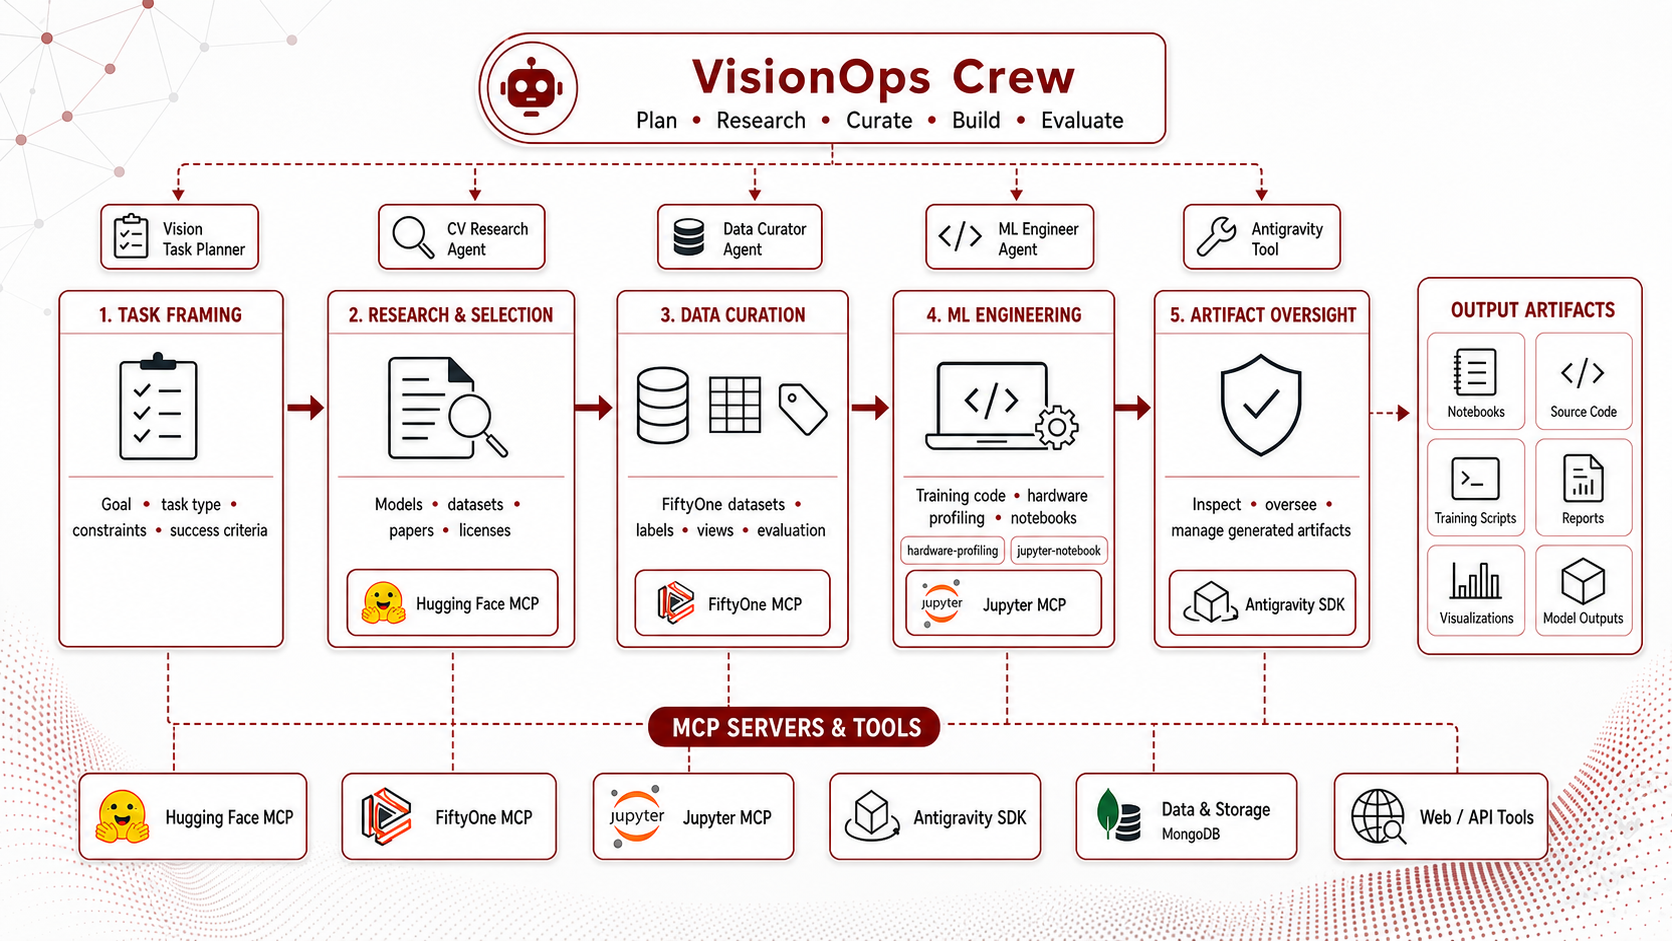
\includegraphics[width=0.75\textwidth]{../../assets/visionops_workflow_artifacts.png}
    \caption{A typical workflow spans discovery, subset loading, data quality checks, baseline selection, and hardware-aware training design. The manual steps between these phases introduce frequent interface-switching overhead and silent schema errors.}
    \label{fig:traditional_pipeline}
\end{figure}

The underlying problem is context isolation. The researcher may understand the dataset schema, the model family, and the runtime constraints, but individual tools do not share that state. \texttt{visionops\_crew} addresses this by routing each stage through specialist agents while keeping the orchestrator responsible for preserving the task brief, evidence, assumptions, and next-step constraints.

\section{System Design: The Multi-Agent Coordinator Architecture}
The system uses a hub-and-spoke architecture. A central ADK app, \texttt{visionops\_crew}, defines a root orchestrator that calls specialist agents as tools. The orchestrator is responsible for task interpretation, routing, context preservation, and synthesis. Specialist agents are responsible for evidence gathering or action within a narrow domain.

This design is intentionally conservative. A single monolithic agent with all tools available can blur responsibilities: the same agent may search the web, mutate local files, inspect datasets, and generate training code without a clear boundary between research, execution, and synthesis. In \texttt{visionops\_crew}, tool access is partitioned by role. This makes prompts easier to audit, reduces accidental tool use, and creates a clearer path for adding confirmation gates around state-changing operations. Figure~\ref{fig:architecture} illustrates the system architecture.

\begin{figure}[htbp]
    \centering
    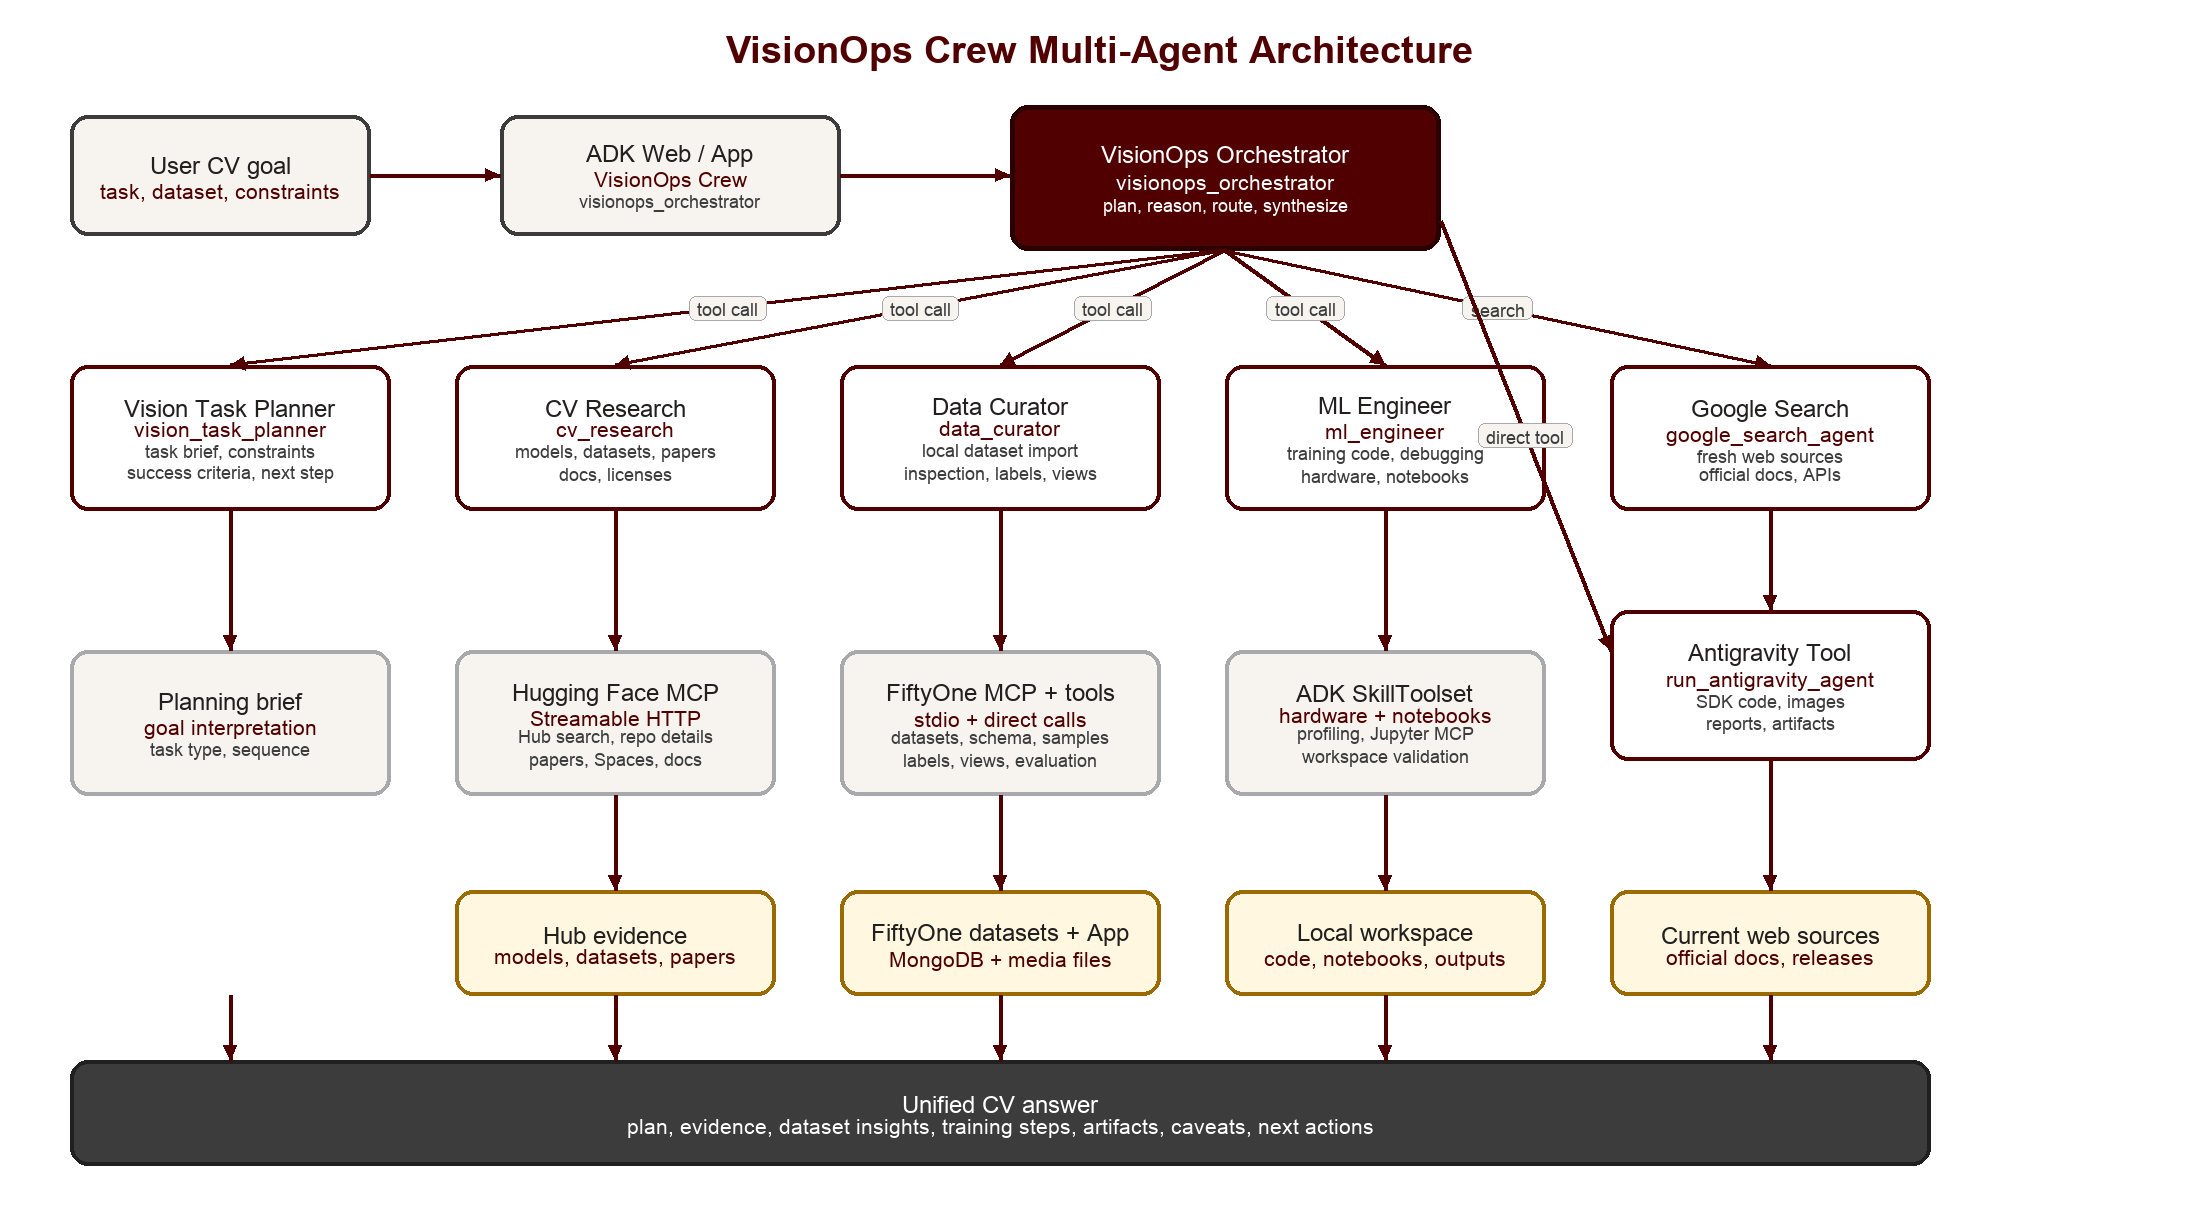
\includegraphics[width=0.95\textwidth]{../../assets/visionops_multi_agent_architecture.png}
    \caption{Multi-agent architecture of \texttt{visionops\_crew}. The orchestrator (\texttt{visionops\_orchestrator}) delegates to specialized sub-agents via standard tool calls, uses MCP servers to bridge external hubs and local runtimes, connects Jupyter MCP through the ML Engineer skill set, and keeps Antigravity SDK as an opt-in direct orchestrator tool.}
    \label{fig:architecture}
\end{figure}

\subsection{Specialist Agents and Their Domains}
The assistant's capabilities are divided among specialist roles. Each role owns a bounded part of the workflow and returns structured findings to the orchestrator:

\begin{enumerate}
    \item \textbf{Vision Task Planner (\texttt{vision\_task\_planner})}: 
    The planner converts broad requests into an operational task brief. It identifies the task type, expected label structure, missing constraints, likely evaluation metrics, execution risks, and the recommended specialist sequence. For research workflows, this creates an explicit hypothesis about what must be observed before implementation should begin. Common CV tasks identified by this planner are shown in Figure~\ref{fig:cv_tasks}.
    
    \begin{figure}[htbp]
        \centering
        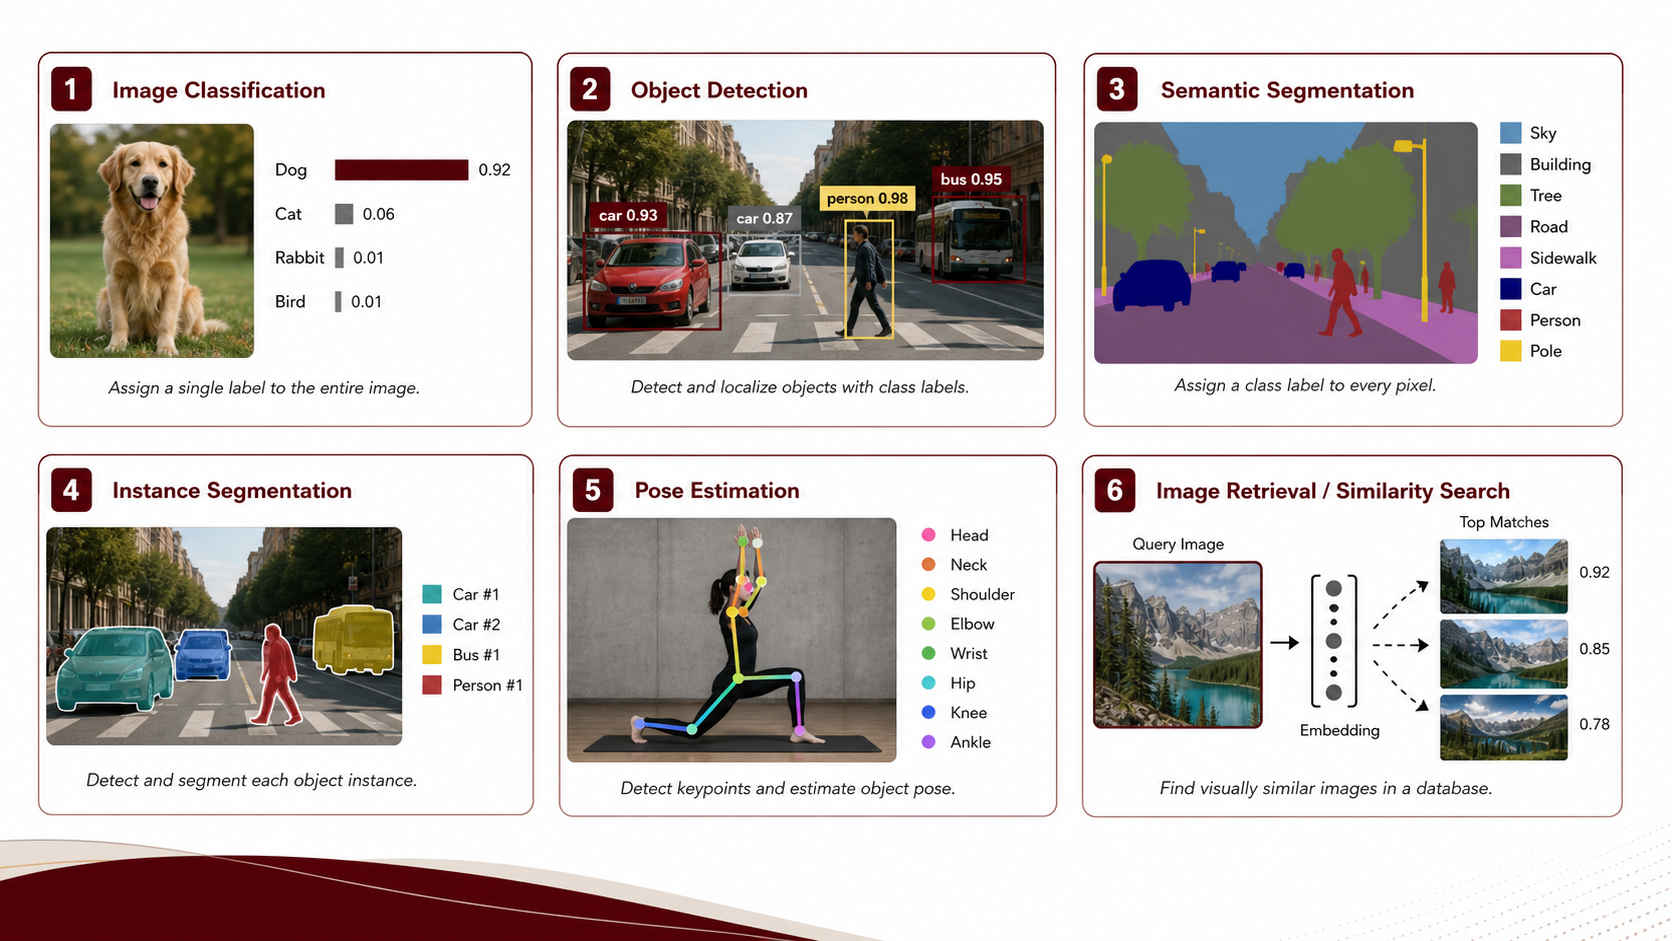
\includegraphics[width=0.8\textwidth]{../../assets/common_cv_tasks.png}
        \caption{Common computer vision tasks recognized by the Vision Task Planner. The identified task type governs downstream actions: Hugging Face model tags, FiftyOne label fields, evaluation metrics, and implementation targets.}
        \label{fig:cv_tasks}
    \end{figure}

    \item \textbf{CV Research Agent (\texttt{cv\_research})}: 
    This specialist is connected to the Hugging Face Hub through MCP. It retrieves datasets, model cards, papers, Spaces, documentation, benchmark context, and licensing metadata. Its output is treated as source-backed research evidence, not as a local execution result.

    \item \textbf{Data Curator Agent (\texttt{data\_curator})}: 
    This agent coordinates local data-centric workflows. It can import Hugging Face datasets into FiftyOne, inspect schemas, summarize label distributions, query samples, and launch the FiftyOne App for visual inspection. Its role is to convert external dataset references into observable local evidence. Using direct tools and a local Stdio MCP session, it manages:
    \begin{itemize}
        \item \texttt{load\_huggingface\_dataset}: Downloads image/video samples from the HF Hub, materializes the assets on the local filesystem (customizable via the \texttt{VISIONOPS\_CREW\_DATASETS\_DIR} environment variable), and builds structured FiftyOne datasets without manual script writing.
        \item \texttt{open\_fiftyone\_dataset}: Launches the interactive FiftyOne App session on a local port to visually inspect labels, flag prediction errors, and display high-dimensional embeddings (using UMAP/t-SNE clusters).
    \end{itemize}

    \item \textbf{ML Engineer (\texttt{ml\_engineer})}: 
    This agent owns implementation-oriented work: hardware-aware training plans, code review, local file inspection, validation commands, and notebook prototyping. It loads two modular ADK skills: \texttt{hardware-profiling} for runtime and accelerator inspection, and \texttt{jupyter-notebook} for durable exploratory work. The notebook skill is backed by the Jupyter MCP gateway, allowing notebooks to be manipulated through structured tool calls rather than loose shell snippets.

    \item \textbf{Google Search Agent (\texttt{google\_search\_agent})}: 
    A freshness-oriented tool for official documentation, releases, API changes, and non-Hugging Face sources.

    \item \textbf{Antigravity Tool (\texttt{run\_antigravity\_agent})}: 
    Antigravity is registered as an opt-in root tool rather than as a default ML Engineer capability. This placement is deliberate: it makes artifact generation, image generation, report drafting, and large implementation tasks explicit user decisions. The wrapper records artifact roots and tool results, denies file writes by default, and only enables create/edit policies after confirmation.
\end{enumerate}

\section{Implementation Details: ADK and MCP Server Integration}
The architecture above is only useful if the boundaries are concrete in code. \texttt{visionops\_crew} implements those boundaries through ADK agent composition, MCP-backed tool registration, local runtime inspection, notebook skills, and explicit artifact controls.

\subsection{Orchestrator Setup}
The root orchestrator, \texttt{visionops\_orchestrator}, is instantiated as a standard ADK \texttt{Agent}. The important design choice is that specialist agents are registered as callable tools via \texttt{AgentTool}. This keeps the user conversation anchored in one root agent while still allowing domain-specific prompts and toolsets behind each specialist. Listing~\ref{lst:orchestrator_setup} shows the simplified initialization pattern:

\begin{lstlisting}[language=Python, caption={Declaring the Orchestrator and registering specialist agents as standard tools using Google ADK.}, label={lst:orchestrator_setup}]
from google.adk.agents import Agent
from google.adk.apps.app import App
from google.adk.plugins import ReflectAndRetryToolPlugin
from google.adk.tools.agent_tool import AgentTool

from visionops_crew.agents.cv_research.agent import (
    root_agent as cv_research,
)
from visionops_crew.agents.data_curator.agent import (
    root_agent as data_curator,
)
from visionops_crew.agents.ml_engineer.agent import (
    root_agent as ml_engineer,
)
from visionops_crew.agents.vision_task_planner.agent import (
    root_agent as vision_task_planner,
)

root_agent = Agent(
    model="gemini-3.5-flash",
    name="visionops_orchestrator",
    description="Main multi-agent orchestrator for computer vision workflows.",
    instruction="""You are a senior computer vision expert. Call the right specialist tools.
    - Call vision_task_planner first to plan ambiguous/multi-step requests.
    - Call cv_research for dataset/model research on HF Hub.
    - Call data_curator for local FiftyOne imports, filtering, and App launches.
    - Call ml_engineer for hardware-aware code, validation, and notebooks.
    - Call run_antigravity_agent only after the user explicitly asks for Antigravity.""",
    tools=[
        AgentTool(agent=vision_task_planner),
        AgentTool(agent=cv_research),
        AgentTool(agent=ml_engineer),
        AgentTool(agent=data_curator),
        run_antigravity_agent,
    ],
)
\end{lstlisting}

\subsection{Integrating External Tools Such as Jupyter, FiftyOne, and Hugging Face through MCP and Skills}
After the orchestrator decides which specialist should act, the next question is how that specialist reaches the right external system. \texttt{visionops\_crew} handles this through MCP toolsets and skills instead of hardcoding platform-specific behavior into the root agent. The boundary stays explicit: tools are discovered from schemas, invoked through ADK, and scoped to the specialist agent that owns the domain. The Hugging Face integration uses a remote MCP gateway for Hub research. The FiftyOne integration launches a local \texttt{fiftyone-mcp} subprocess over stdio so it can inspect datasets in the same Python environment as the ADK app.

\begin{lstlisting}[language=Python, caption={Configuring a local Stdio MCP session for FiftyOne in \texttt{data\_curator/agent.py}.}]
from pathlib import Path
import sys
from google.adk.tools.mcp_tool.mcp_toolset import McpToolset
from google.adk.tools.mcp_tool.mcp_session_manager import (
    StdioConnectionParams,
    StdioServerParameters,
)

fiftyone_mcp_path = Path(sys.executable).with_name("fiftyone-mcp")

fiftyone_mcp_tools = McpToolset(
    connection_params=StdioConnectionParams(
        server_params=StdioServerParameters(
            command=str(fiftyone_mcp_path),
            env=dict(os.environ),
            cwd=str(Path(__file__).resolve().parent.parent),
        ),
        timeout=30.0,
    ),
)
\end{lstlisting}

The \texttt{McpToolset} class queries the MCP server's tool schemas and registers the resulting operations inside the ADK agent's scope. In practice, this means the Data Curator can inspect local dataset state while the orchestrator remains focused on routing and synthesis, not on the details of FiftyOne's SDK calls.

\subsection{Local Hardware and Framework Auditing}
Once data and model context are available, implementation advice still has to match the runtime. Hardware and framework state is therefore a first-class part of the workflow because it constrains feasible baselines. A recommendation that ignores memory, accelerator support, or installed framework versions is incomplete. The \texttt{ml\_engineer} uses a modular ADK skill named \texttt{hardware-profiling} to inspect the platform visible to the ADK runtime. By invoking \texttt{scripts/profiling\_tools.py} through the skill boundary, the agent checks CPU details, memory, framework availability, and accelerator support before proposing training parameters. Listing~\ref{lst:profiling_tools} shows the helper implementations in the skill script:

\begin{lstlisting}[language=Python, caption={Auditing device specifications, frameworks, and accelerators in the \texttt{hardware-profiling} skill script.}, label={lst:profiling_tools}]
def check_hardware_specification() -> dict:
    """Inspect local CPU, memory, and operating system platform details."""
    info = {
        "platform": {
            "system": platform.system(),
            "release": platform.release(),
            "machine": platform.machine(),
            "processor": platform.processor(),
            "python": platform.python_version(),
            "python_executable": os.sys.executable,
        },
        "cpu": {"logical_cores": os.cpu_count()},
        "memory": {}
    }
    if platform.system() == "Darwin" and shutil.which("sysctl"):
        memsize = subprocess.run(["sysctl", "-n", "hw.memsize"], capture_output=True, text=True).stdout.strip()
        if memsize.isdigit():
            info["memory"]["total_gb"] = round(int(memsize) / (1024**3), 2)
    return info

def check_framework_availability() -> dict:
    """Inspect availability and versions of major ML and DL frameworks."""
    # Dynamic checks for torch, jax, sklearn, tensorflow, transformers, timm, fiftyone...
    ...

def check_accelerator_availability() -> dict:
    """Inspect availability of hardware accelerators (CUDA/MPS/TPUs)."""
    # Checks nvidia-smi command and framework-specific device listings...
    ...
\end{lstlisting}

This profiling does not claim to characterize the user's entire deployment environment; it characterizes the runtime that the agent can actually observe. The distinction matters for researchers who prototype locally but train on remote clusters. In those cases, the target hardware must be supplied explicitly in the task brief.

\subsection{Interactive Prototyping with Jupyter Notebooks}
After the runtime has been inspected, the ML Engineer can use notebooks for exploratory checks without losing provenance. Notebook workflows are treated as structured artifacts rather than temporary scratch space. The \texttt{ml\_engineer} manages notebooks through the \texttt{jupyter-notebook} skill and a Stdio-based MCP server connected to \texttt{jupyter-mcp-server@latest}. This allows the agent to create, open, edit, execute, and inspect notebook cells while preserving the notebook as an auditable artifact.

When starting exploratory work or training script verification, the agent creates or loads a notebook (e.g., \texttt{pytorch\_image\_classifier.ipynb}) and inserts cells incrementally. Listing~\ref{lst:notebook_creation} shows how the orchestrator configures the Jupyter MCP tool wrapper in ADK:

\clearpage

\begin{lstlisting}[language=Python, caption={Registering the Jupyter MCP server over stdio in \texttt{ml\_engineer/agent.py}.}, label={lst:notebook_creation}]
from google.adk.tools.mcp_tool.mcp_toolset import McpToolset
from google.adk.tools.mcp_tool.mcp_session_manager import (
    StdioConnectionParams,
    StdioServerParameters,
)

jupyter_mcp_toolset = McpToolset(
    connection_params=StdioConnectionParams(
        server_params=StdioServerParameters(
            command="uvx",
            args=["jupyter-mcp-server@latest"],
            env=dict(os.environ)
        ),
        timeout=30.0
    )
)
\end{lstlisting}

Cell-level MCP tools such as \texttt{insert\_cell}, \texttt{edit\_cell\_source}, \texttt{execute\_cell}, and \texttt{list\_kernels} allow the agent to build prototypes incrementally. For research workflows, this is useful because intermediate diagnostics such as class histograms, sample grids, and training curves can stay attached to the code that produced them.

\subsection{Antigravity SDK as an Opt-In Orchestrator Tool}
The previous sections describe the default path for research, data inspection, runtime checks, and notebooks. Antigravity sits outside that default path. Its SDK integration is intentionally placed at the root orchestrator boundary so normal CV routing remains predictable: model research still goes through the CV Research agent, local dataset work still goes through the Data Curator, and notebook prototyping still belongs to the ML Engineer. Antigravity is reserved for requests where a stronger implementation assistant is useful, such as generating an image asset, drafting a validation report, inspecting a project structure, or producing a proposed notebook or script.

The standalone demo in \texttt{scripts/antigravity\_sdk\_demo.py} shows the core SDK pattern. First, the local agent is configured with repo-local workspace and session directories:

\begin{lstlisting}[language=Python, caption={Creating a local Antigravity SDK configuration from \texttt{scripts/antigravity\_sdk\_demo.py}.}, label={lst:antigravity_config}]
from google.antigravity import Agent, LocalAgentConfig
from google.antigravity.hooks import policy

config = LocalAgentConfig(
    system_instructions=(
        ANTIGRAVITY_EXPERT_INSTRUCTIONS
    ),
    model=os.getenv("ANTIGRAVITY_MODEL", "gemini-3.5-flash"),
    workspaces=[str(REPO_ROOT)],
    api_key=os.getenv("GEMINI_API_KEY"),
    save_dir=str(
        ANTIGRAVITY_SESSIONS_DIR / "expert"
    ),
    app_data_dir=str(ANTIGRAVITY_APP_DATA_DIR),
    policies=[
        policy.ask_user(
            "generate_image",
            handler=interactive.ask_user_handler,
            name="allow-gen",
        ),
        policy.confirm_run_command(handler=interactive.ask_user_handler),
    ],
)
\end{lstlisting}

\clearpage

Then a task is executed as an asynchronous chat turn:

\begin{lstlisting}[language=Python, caption={Running one Antigravity task as an async SDK call.}, label={lst:antigravity_run}]
async with Agent(config) as agent:
    response = await agent.chat(task)
    result = await response.text()
\end{lstlisting}

Inside the ADK app, \texttt{run\_antigravity\_agent} wraps this SDK flow with stricter policies: file creation and editing are denied unless the user has confirmed the exact write action, shell command execution is denied in the non-interactive tool path, generated images are allowed, and created or updated artifacts are reported from concrete configured roots. This turns Antigravity into a controlled extension of \texttt{visionops\_crew}, not a hidden side channel.

\section{End-to-End Walkthrough: An Audited Curation and Training Plan}
With the implementation pieces in place, the full value of the architecture appears when a request spans several systems. Consider a request that requires local data work and implementation guidance:
\begin{quote}
    \textit{``Load Humayoun/SkinDisease into FiftyOne, inspect the label schema, and suggest a baseline image classification training plan for my local hardware.''}
\end{quote}

Figure~\ref{fig:workflow_trace} illustrates the multi-agent execution flow.

\begin{figure}[htbp]
    \centering
    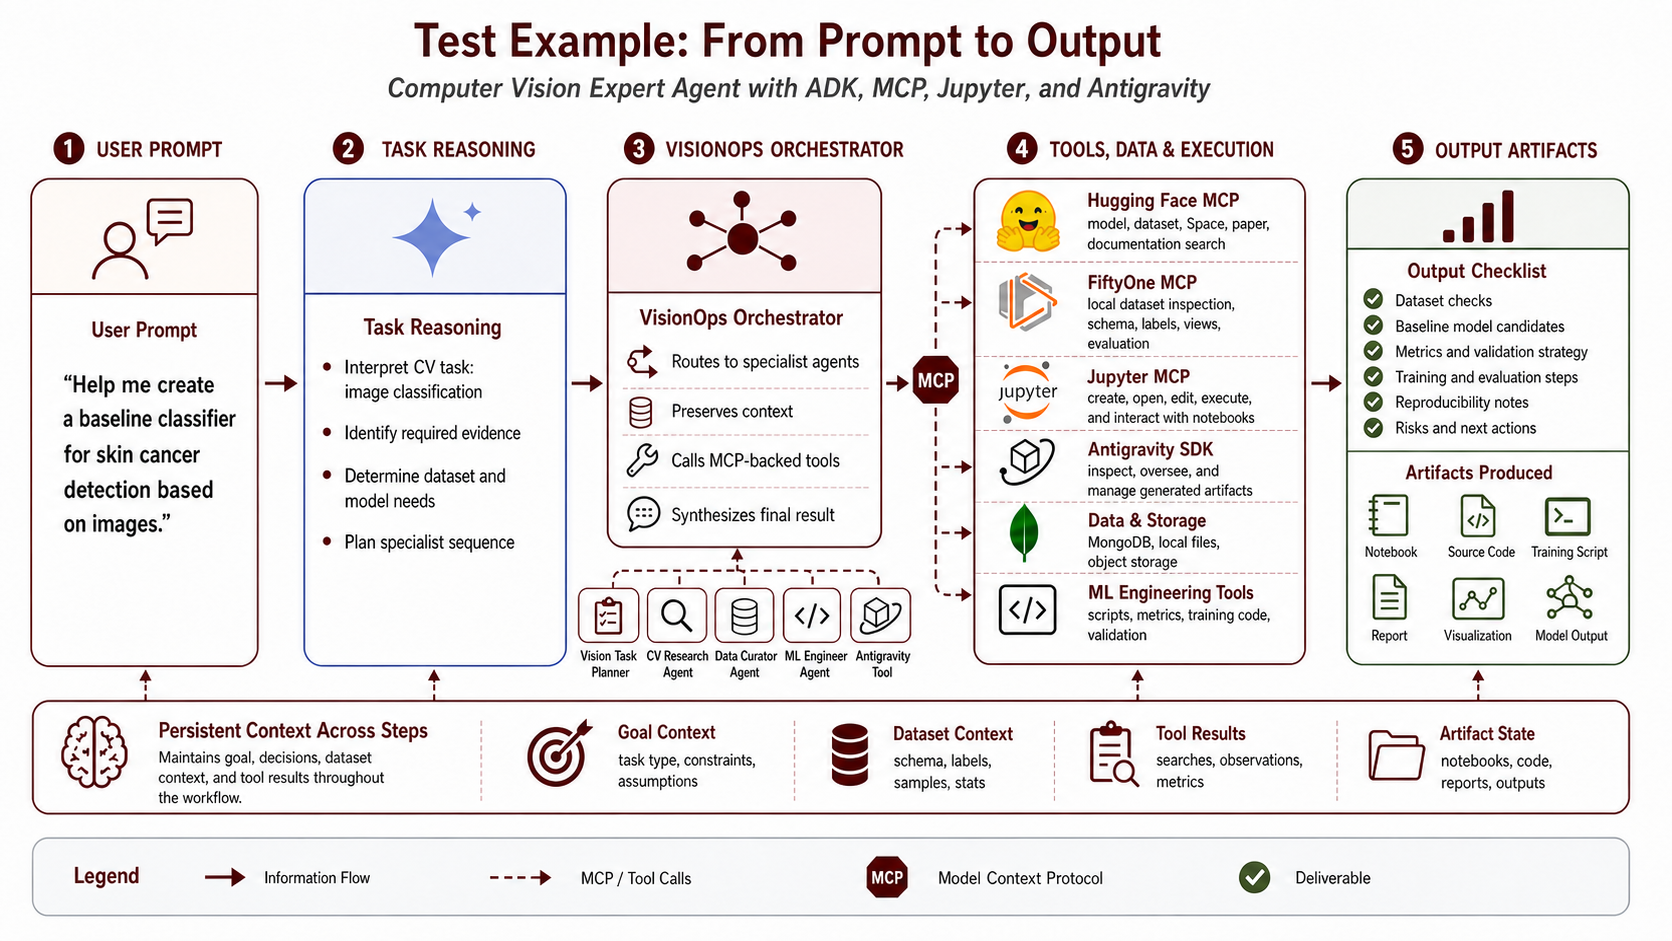
\includegraphics[width=0.9\textwidth]{../../assets/test_example_prompt_to_output.png}
    \caption{Prompt-to-output workflow trace. The orchestrator plans the steps, routes research and local inspection through MCP-backed tools, uses Jupyter MCP for notebook-capable ML engineering, and can invoke Antigravity only when explicitly requested for implementation or artifact-generation work.}
    \label{fig:workflow_trace}
\end{figure}

The workflow is intentionally sequential. The system first establishes task and data evidence, then uses that evidence to guide implementation:
\begin{enumerate}
    \item \textbf{Task framing}: The orchestrator calls \texttt{vision\_task\_planner}. The planner identifies the request as image classification, records missing constraints, and recommends dataset inspection before training advice.
    \item \textbf{Data ingestion}: The orchestrator invokes \texttt{data\_curator} using the custom \texttt{load\_huggingface\_dataset} tool to request a bounded sample of the \texttt{Humayoun/SkinDisease} repository. The agent materializes media under the configured dataset directory, creates a persistent FiftyOne dataset, and can launch the App for visual inspection.
    \item \textbf{Schema inspection}: The Data Curator runs local schema and aggregation queries. The goal is to identify the image field, label field, class cardinality, and any immediate imbalance or missing-label issues before generating training code.
    \item \textbf{Hardware and framework audit}: The orchestrator calls the ML Engineer agent only after the data context is known. The agent inspects the runtime and reports:
    \begin{itemize}
        \item \textbf{OS}: macOS (Darwin)
        \item \textbf{Processor}: Apple Silicon M-series
        \item \textbf{Backend Available}: PyTorch MPS (Metal Performance Shaders) device support
    \end{itemize}
    \item \textbf{Synthesis}: The orchestrator combines the planner brief, dataset evidence, and runtime observations into an implementation plan. For example, on Apple Silicon it can recommend a PyTorch transfer-learning baseline using \texttt{device = 'mps'} rather than assuming CUDA.
\end{enumerate}

\section{System Limitations and Safety Constraints}
The walkthrough shows how the system keeps evidence connected, but the architecture still has operational and scientific limits:
\begin{itemize}
    \item \textbf{Latency and cost}: Delegating through multiple agents increases token usage and wall-clock latency. The architecture is most appropriate when the task spans multiple systems or requires auditable evidence, not when a single lookup is sufficient.
    \item \textbf{Local side effects}: Dataset imports, notebook execution, file writes, and command execution can change local state. These actions should remain behind explicit confirmation and should be logged as part of the workflow.
    \item \textbf{Runtime observability}: Hardware inspection only describes the environment visible to the ADK runtime. It does not infer remote training infrastructure unless the user provides that target environment.
    \item \textbf{Scientific validity}: The system can organize evidence and generate baselines, but it cannot guarantee dataset suitability, absence of bias, statistical power, clinical validity, or deployment readiness. Those remain domain-specific research responsibilities.
    \item \textbf{Tool and schema drift}: MCP servers, external APIs, model cards, and dataset schemas can change. Reproducible workflows should record dataset versions, sample sizes, model revisions, and local package versions when results matter.
\end{itemize}

\section{Conclusion and Future Directions}
\texttt{visionops\_crew} demonstrates a practical pattern for agentic computer vision operations: keep orchestration centralized, keep specialist tool access narrow, and make local execution boundaries explicit. The result is not a replacement for experimental judgment; it is a coordination layer that helps preserve context across model research, dataset inspection, runtime profiling, notebook prototyping, and artifact generation.

Future work should focus on stronger reproducibility and evaluation. Useful extensions include recording structured provenance for dataset imports, storing model and dataset revision metadata, integrating FiftyOne similarity search for anomaly discovery, adding benchmark-specific evaluation templates, and supporting closed-loop training runs where failures are diagnosed without hiding execution details from the user.

\end{document}
